\pagebreak
\section{Benutzerhandbuch}

\subsection{Installation}
Um die Applikation zu installieren muss die .apk Installationsdatei zuerst auf das Smartphone übertragen werden. Danach muss sichergestellt werden dass in den Android Einstellungen unter Sicherheit die Option \enquote{Unbekannte Herkunft zulassen} aktiviert wurde. Nun kann mit einem gängigen Dateiexplorer die Installationsdatei geöffnet werden um den Installationsvorgang zu beginnen.

\subsection{Logininformationen hinterlegen}

Um die Applikation verwende zu können müssen die Logininformationen des Benutzers hinterlegt werden. Dazu wird direkt nach dem Start der Applikation das Zahnrad im oberen rechten Ecken berührt.

\begin{wrapfigure}{l}{5.5cm}
	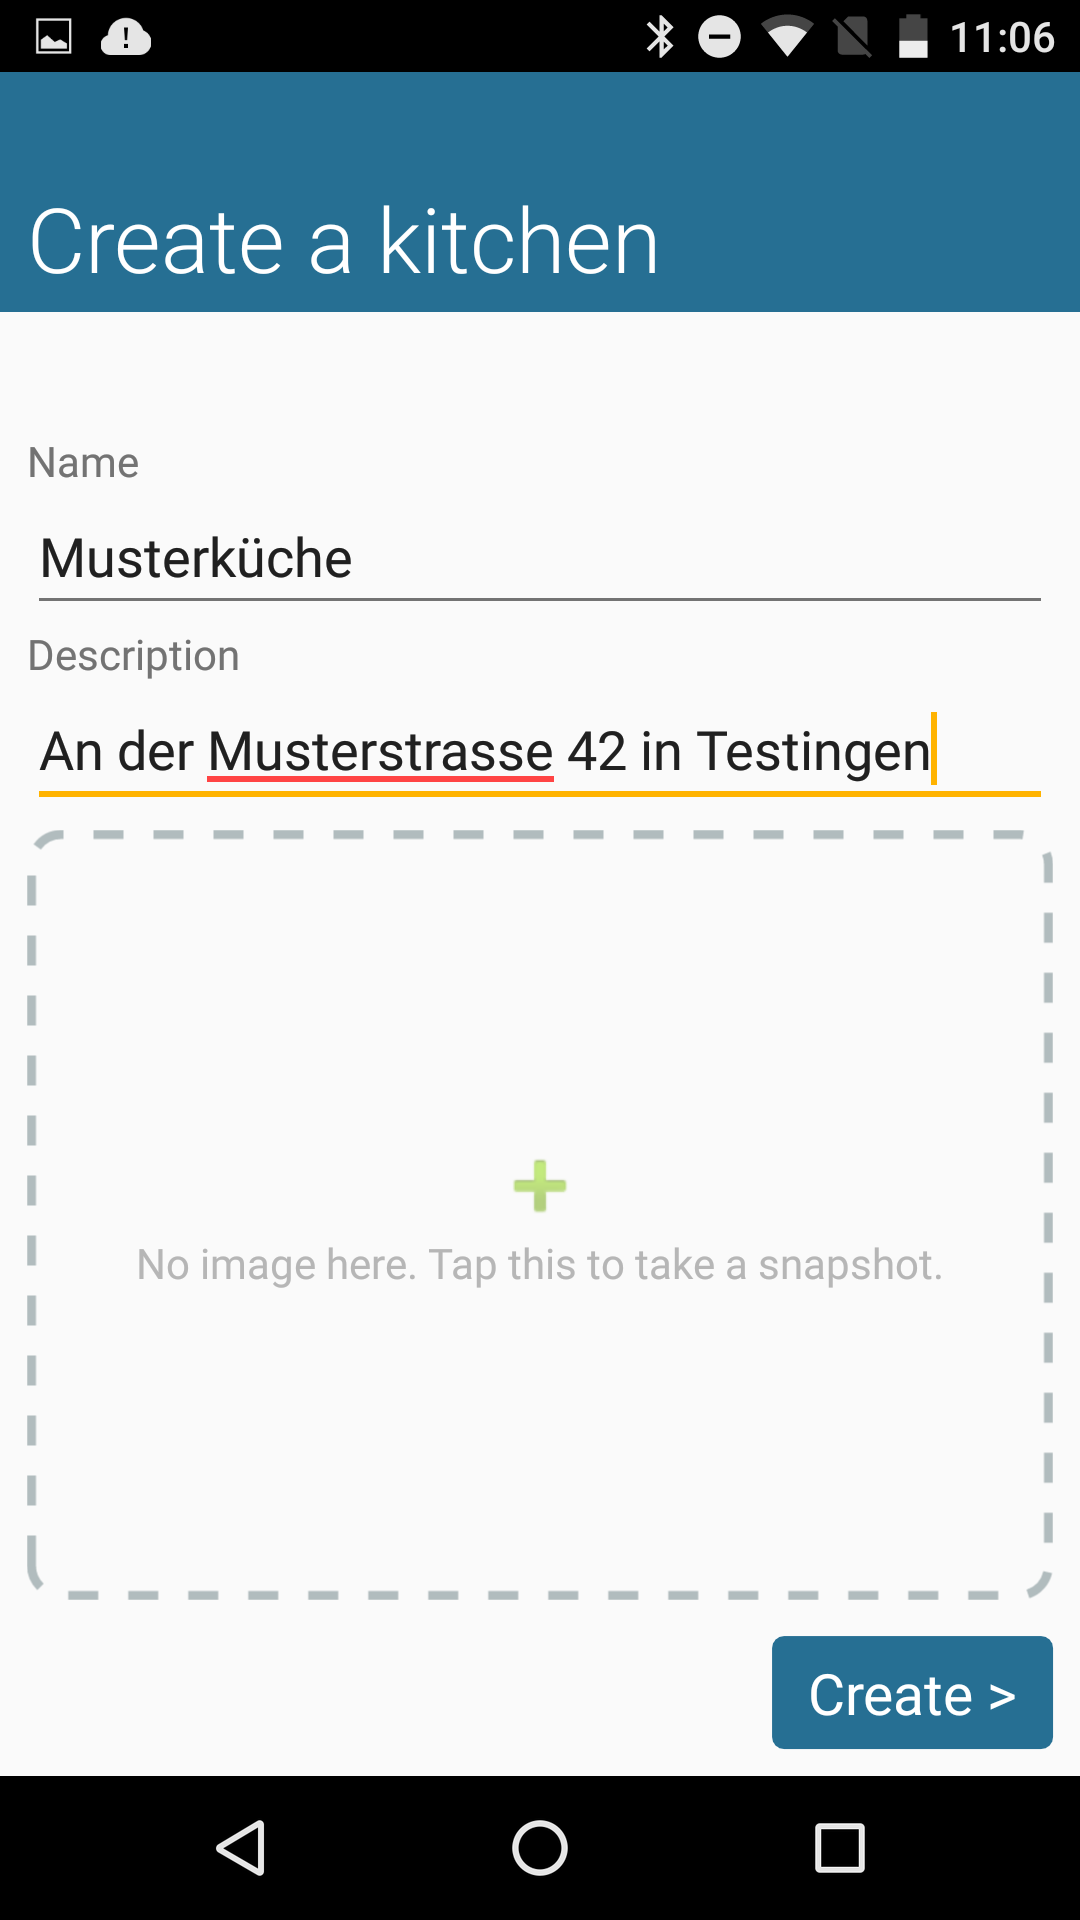
\includegraphics[scale=0.13]{results/res/create_kitchen}
	\caption{Küche erstellen}
\end{wrapfigure}
Dies öffnet die Applikationseinstellungen wo der Nutzername und das Passwort eingegeben werden können.\footnote{Zu Testzwecken kann der Benutzername: \enquote{user} und das Passwort: \enquote{1234} verwendet werden.}

\subsection{Küche erfassen}
Um eine Küche zu erfassen berührt man den \acl{FAB} in der unteren rechten Ecke der Ansicht \enquote{Find a kitchen}. Danach wir der Name der Küche sowie eine optionale Beschreibung erfasst. Zum Schluss wird noch ein Photo der Küche erstellt um eine schneller Wiedererkennung zu ermöglichen.

Nun können für die neu erstellte Küche verschiedene Küchenbereiche erfasst werden. Dazu wird in der aktuellen Ansicht der \acl{FAB}

\WFclear
in der unteren rechten Ecke berührt. Dies kann so lange wiederholt werden bis alle Bereich der Küche erfasst wurden. 

\subsection{Suchlauf durchführen}

Nachdem eine Küche mit mindestens einem Küchenbereich erfasst wurde können Geräte auf dem Bereich platziert werden. Dazu berührt man zuerst das Bild eines Küchenbereichs. Um in diesem Bereich nun ein Suchlauf durchzuführen muss das Bluetooth Symbol in der oberen rechten Ecke berührt werden. Dies öffnet eine Liste welche nun laufend mit den gefunden Geräte befüllt wird. 

\begin{wrapfigure}{l}{5.5cm}
	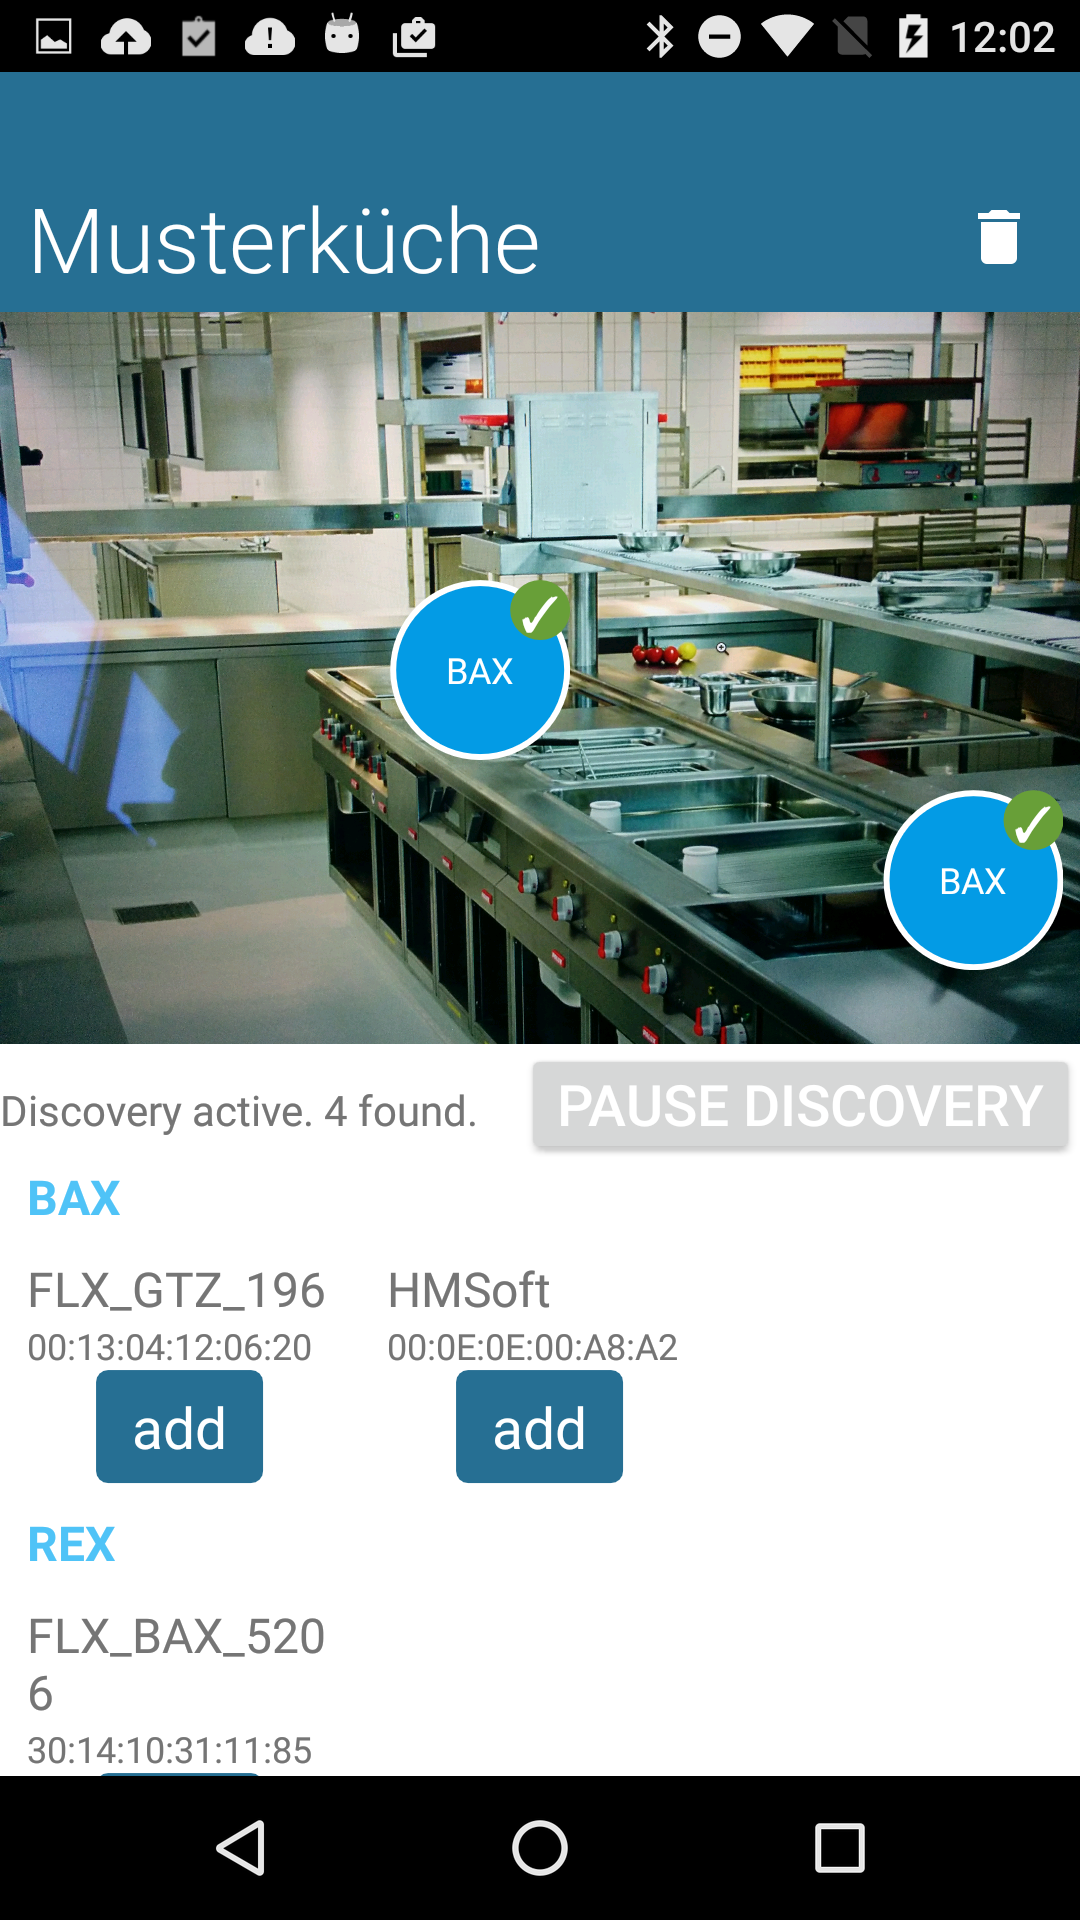
\includegraphics[scale=0.13]{results/res/device_discovery}
	\caption{Geräteerkennung}
\end{wrapfigure}

Geräte mit denen noch keine Verbindung bestand zeigen den Button \enquote{Pair} an. Damit wird der Bonding-Vorgang gestartet welcher kurzzeitig ein Pop-Up für eine Passworteingabe anzeigt. Bei Geräten die mit dem Default Passwort \enquote{1234} konfiguriert sind muss nichts weiter gemacht werden, das Pop-Up verschwindet nach einigen Sekunden automatisch und der Button zeigt daraufhin \enquote{Add} an.

Nach dem Bonding-Vorgang können Geräte auf dem Küchenbereich platziert werden. Dazu berührt man den \enquote{Add} Button worauf das Gerät in der Mitte der Ansicht erscheint. Das Gerät kann auf der Ansicht frei verschoben werden so dass es mit der Einrichtung der Küche übereinstimmt. 

Sobald alle Geräte erfolgreich platziert wurden kann der \enquote{Discovery Modus} mit dem Backbutton des Smartphones verlassen werden.

\WFclear
\subsection{Gerätestatus abrufen}
Um den Status eines Geräts abzurufen muss man sich in der Küchenbereichsansicht befinden. Danach öffnet eine Berührung des gewünschten Geräts die Geräteansicht. Hier hat man die Wahl zwischen vier Tabs: Status, Usage, Errors und Config.

%\begin{wrapfigure}{l}{5.5cm}
%	\vspace{0.7cm}
%	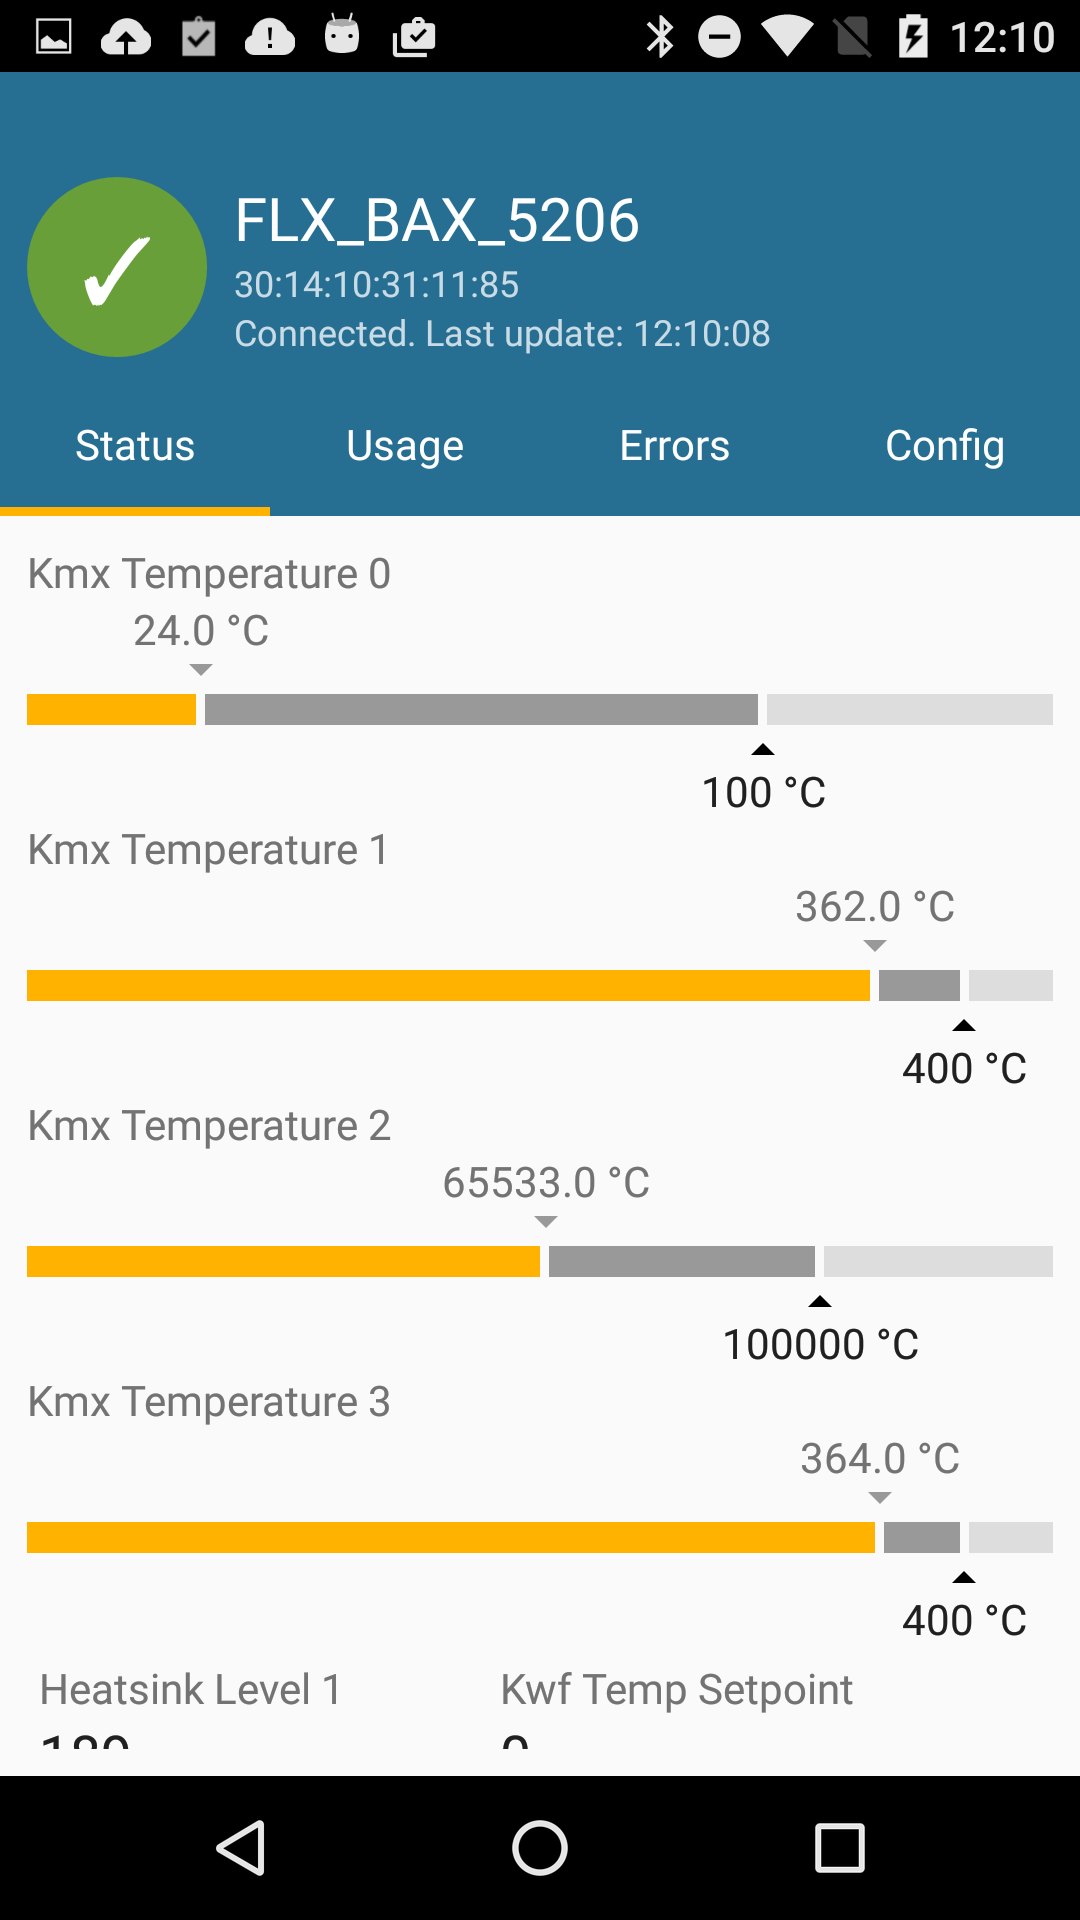
\includegraphics[scale=0.13]{results/res/device_status}
%	\caption{Gerätestatus}
%\end{wrapfigure}

\begin{figure}[h!]
\centering
    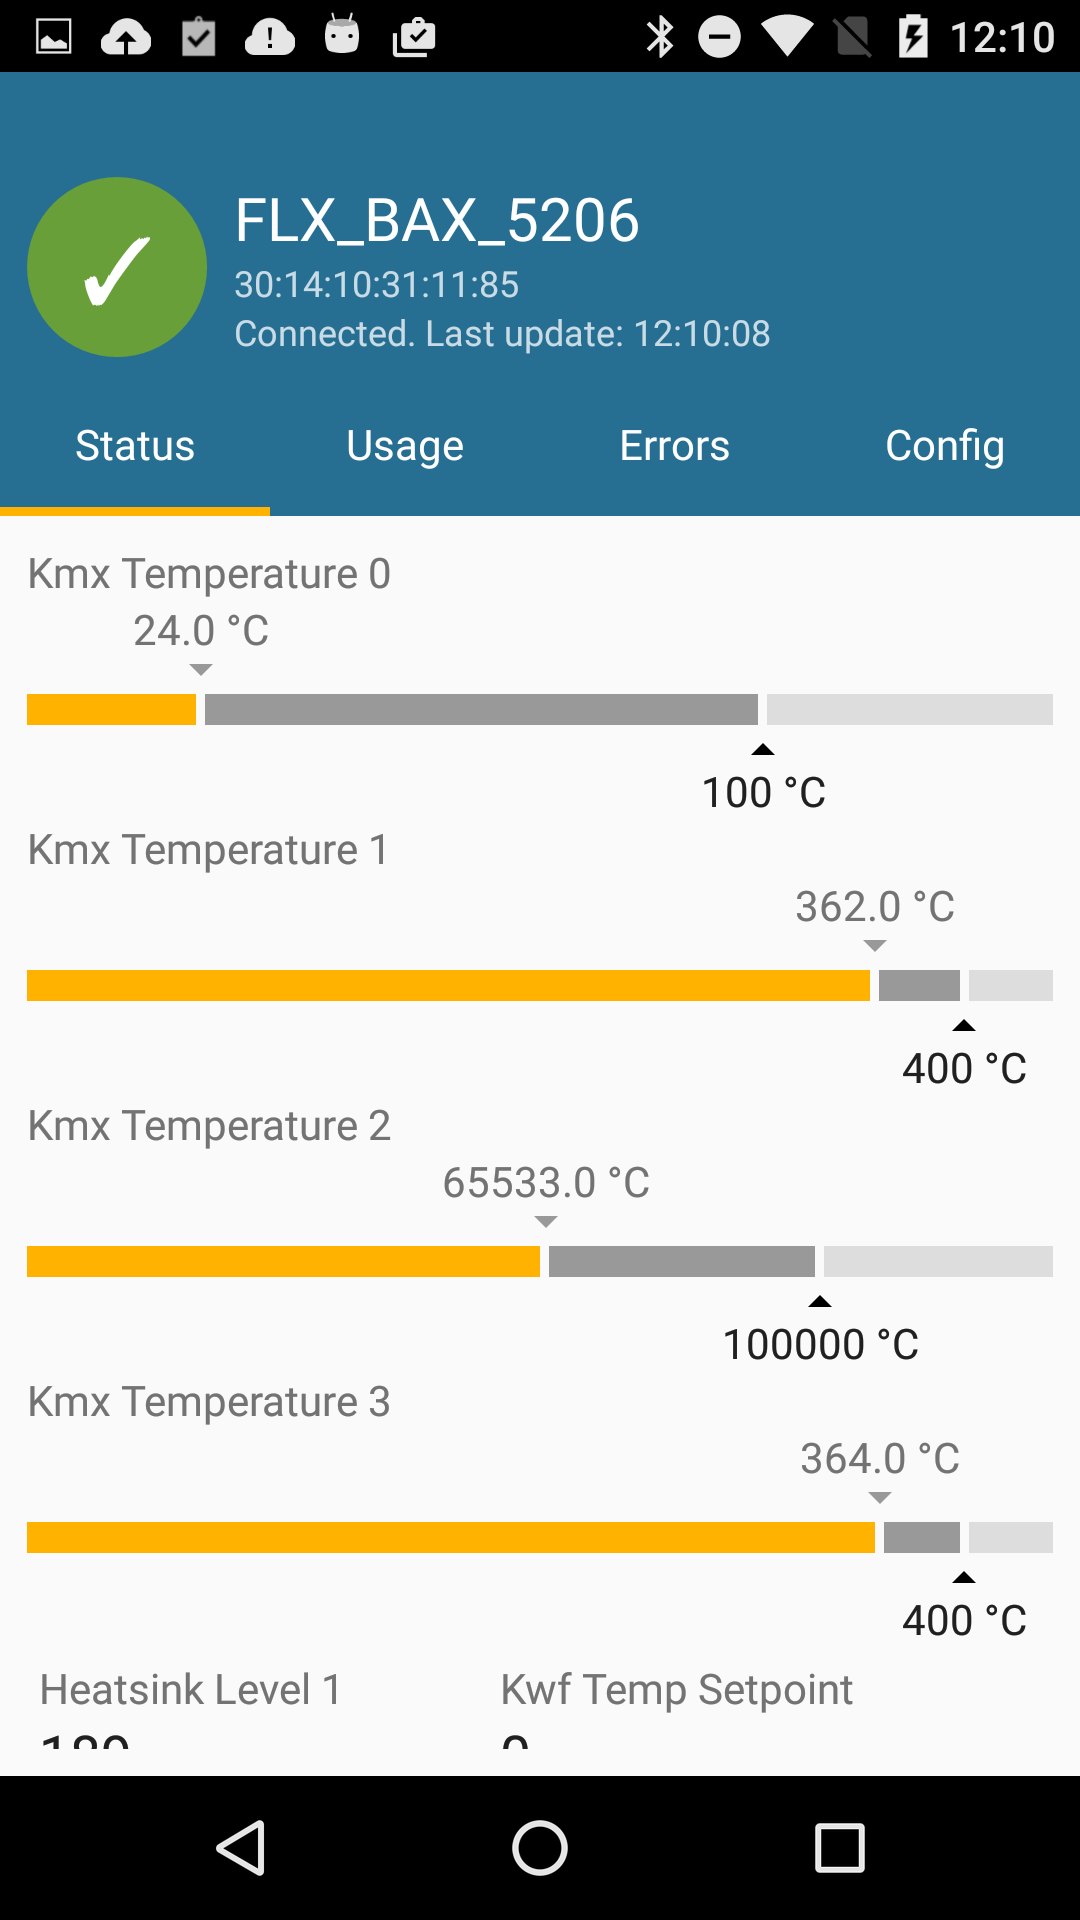
\includegraphics[scale=0.09]{results/res/device_status}
    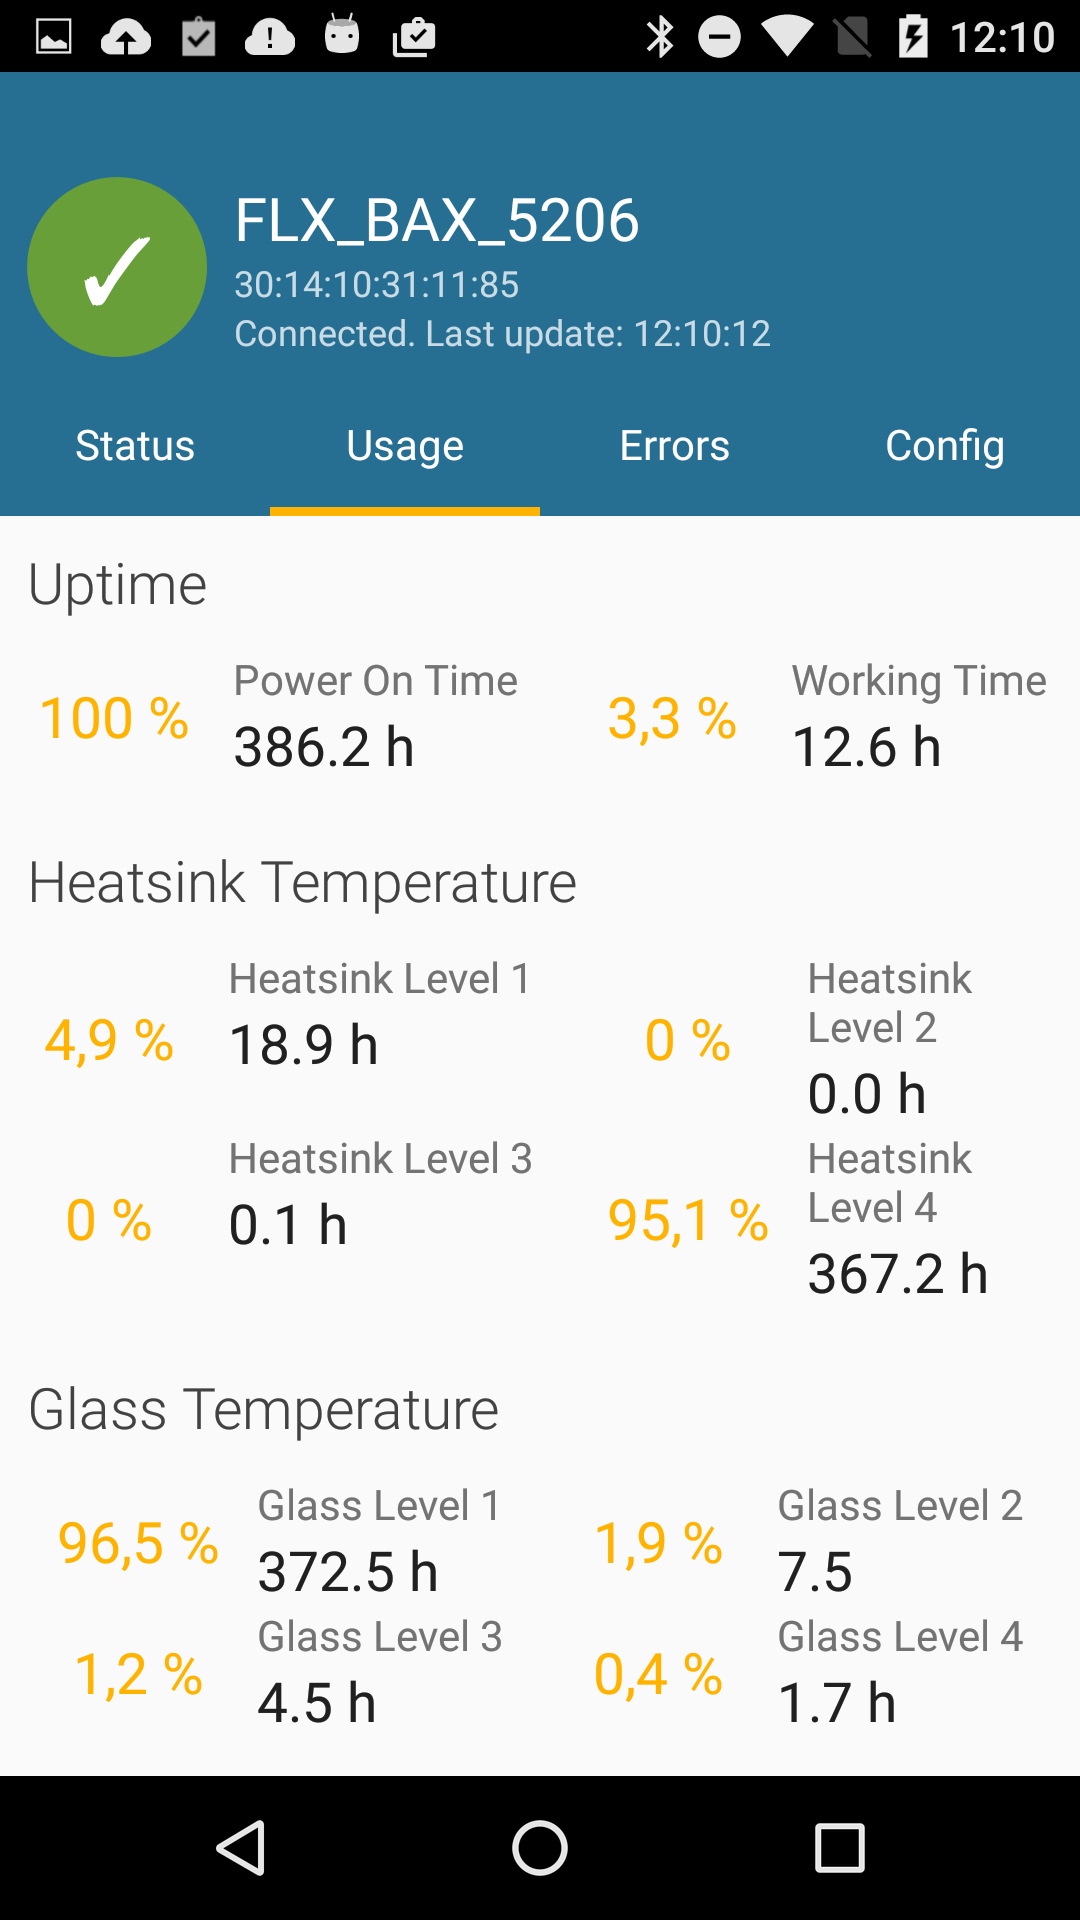
\includegraphics[scale=0.09]{results/res/device_usage}
    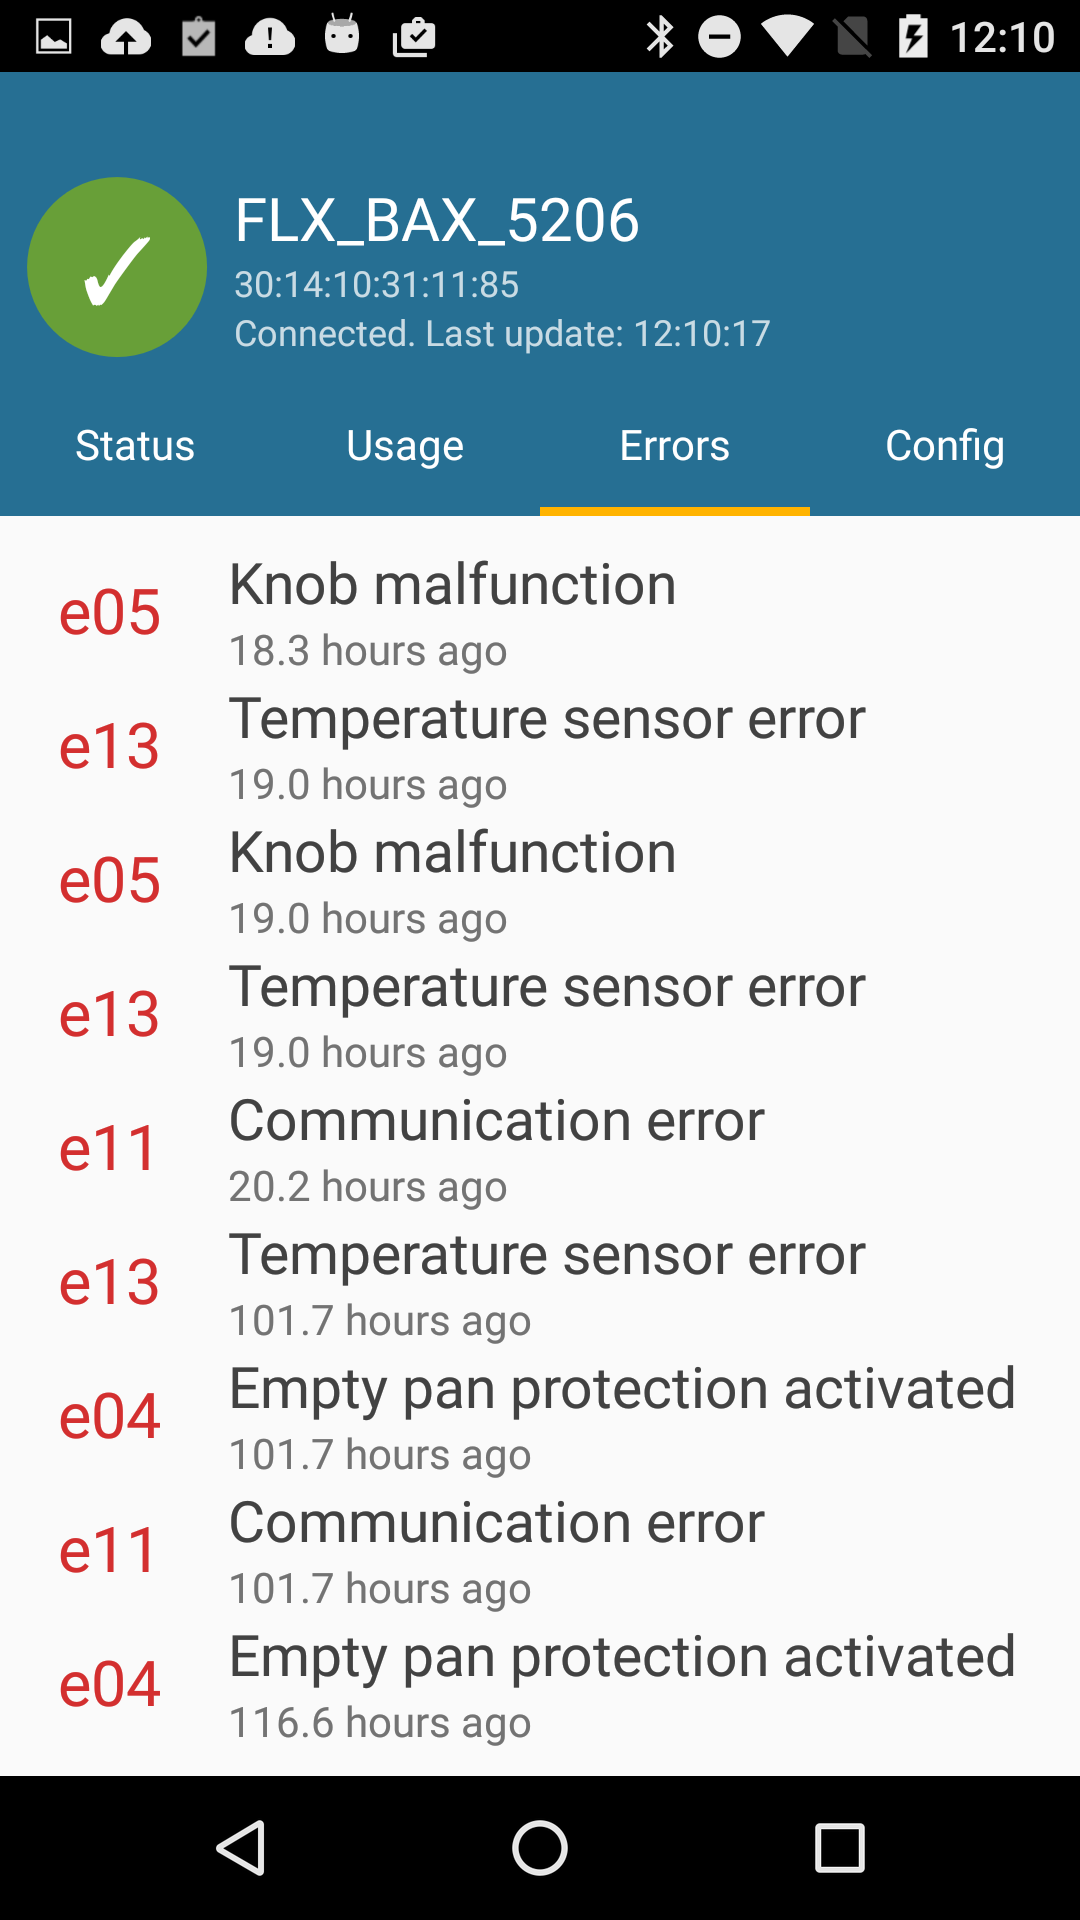
\includegraphics[scale=0.09]{results/res/device_errors}
    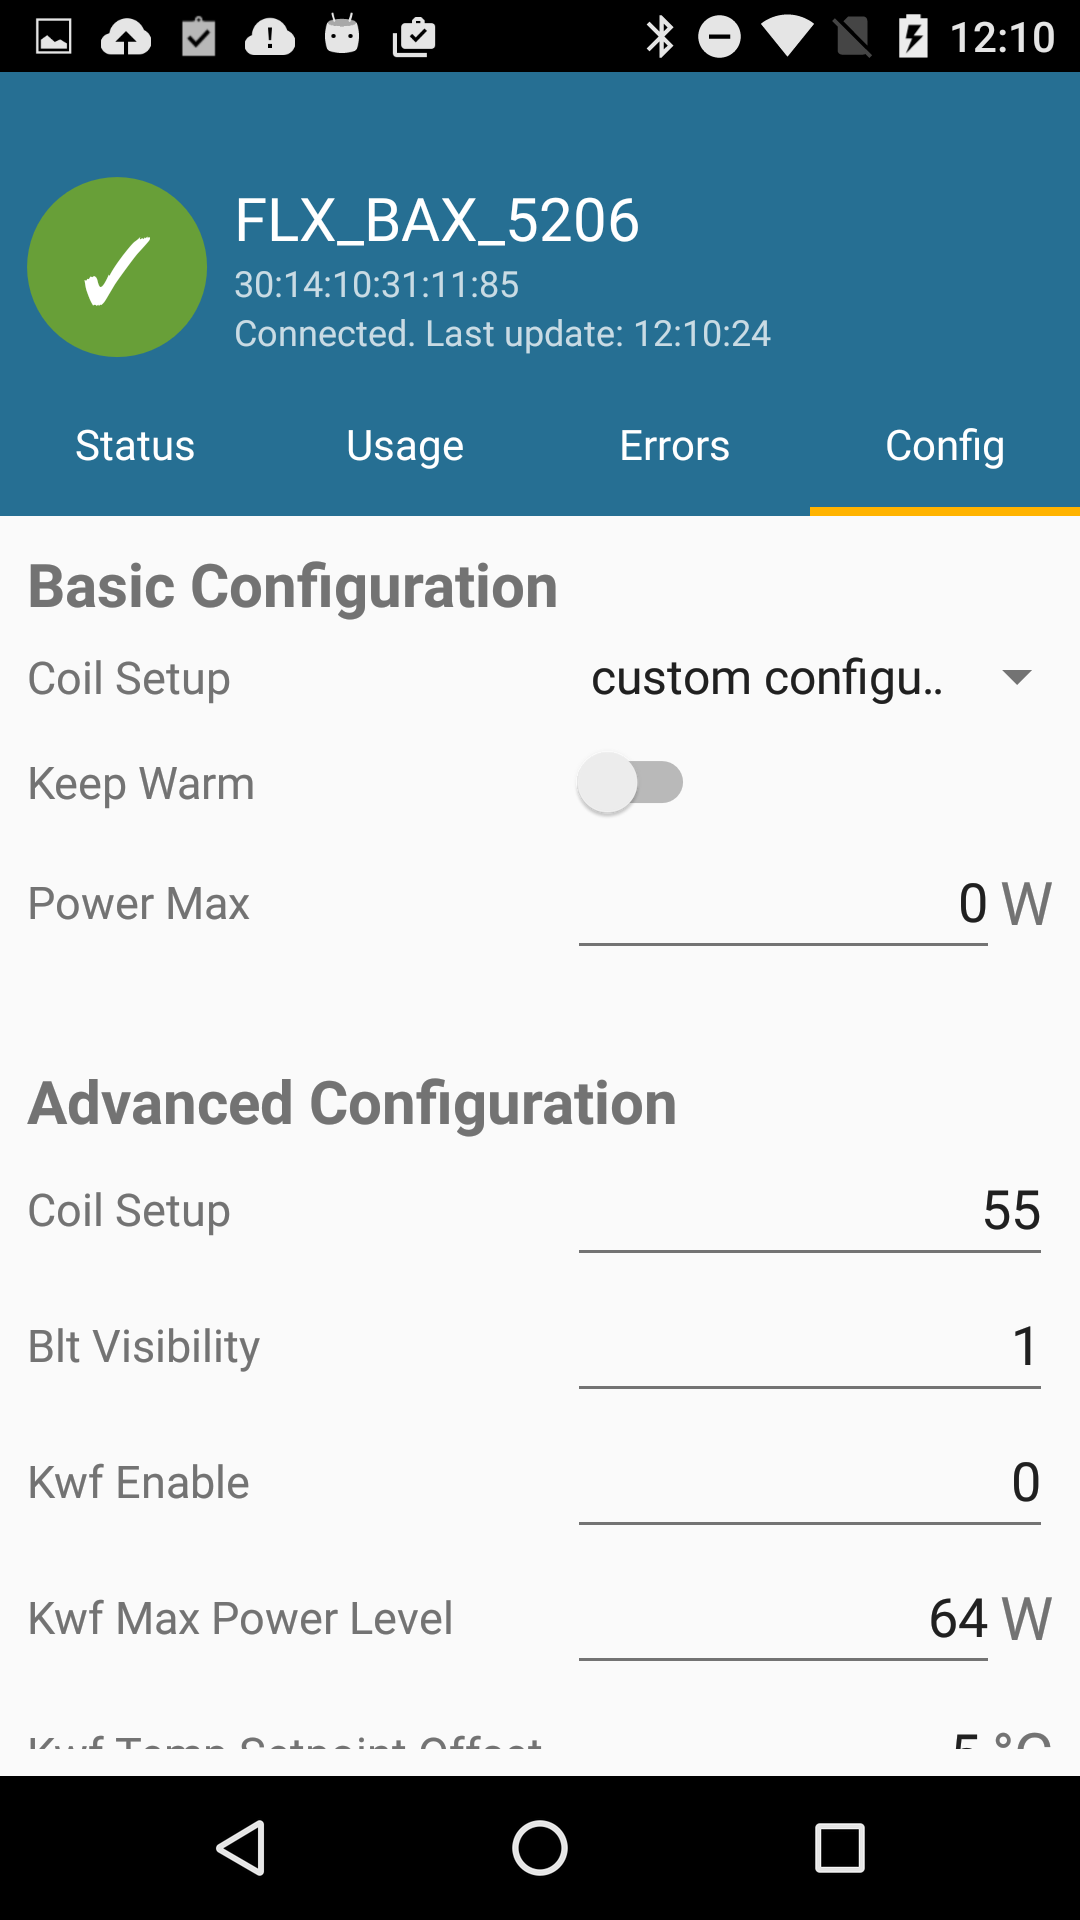
\includegraphics[scale=0.09]{results/res/device_config}
    \caption{Geräte-Detailansicht}
\end{figure}

\begin{itemize}
\item \textbf{Status:}
In der Statusansicht wird die aktuelle Temperatur aller angeschlossenen Sensoren angezeigt. \\
\item \textbf{Usage:}
Unter Usage findet man die Uptime des Geräts sowie die Benutzungsdauer einiger der wichtigsten Komponenten. \\

\item \textbf{Errors:}
Der Tab Errors zeigt eine Liste der Fehler die auf dem Gerät aufgetreten sind. \\

\item \textbf{Config:}
Unter Config können Geräteinstellungen eingesehen und verändert werden. Config ist in eine Überschrift \enquote{Basic Configuration} mit nur den nötigsten Einstellungen sowie \enquote{Advanced Config} mit allen Einstellungen gegliedert.
\end{itemize}

\WFclear
\subsection{Küche editieren}
\label{subsec:kuecheEditieren}
Ausgehend vom Screen \enquote{Find a kitchen} wird eine Küche gewählt und dann auf das Zahnrad im oberen rechten Ecken gedrückt. Dies öffnet die Kücheneinstellung worin der Name und die Beschreibung der Küche geändert werden können. Änderungen werden automatisch gespeichert.

\subsection{Küche exportieren}
\label{subsec:kuecheExportieren}
Um eine Küche zu exportieren muss zuerst zu den Kücheneinstellungen navigiert werden. Siehe \ref{subsec:kuecheEditieren}. Dort kann via dem Button \enquote{Share via EMail} der Export-Vorgang gestartet werden. Nachdem die Applikation den Export zusammengestellt hat erscheint eine Auswahl von Applikationen mit denen die exportierte Küche versendet oder gespeichert werden kann. Wenn zum Beispiel Gmail gewählt wird, wird die exportierte Küche als .fluxron Datei angehängt. 

\subsection{Küche importieren}
Um eine Küche zu importierten benötigt man eine .fluxron Datei. Siehe \ref{subsec:kuecheExportieren}. Diese Datei kann auf ein Smartphone via File Transfer übertragen und dann mit einem herkömmlichen Datei Explorer geöffnet werden. Alternativ kann man sich Datei auch als EMail Anhang zusenden und direkt aus der Mail Applikation heraus öffnen.

\subsection{Deinstallation}
Die Deinstallation erfolgt durch ein langes Drücken des Applikations-Icons. Das Icon kann dann auf den Mülleimer gezogen werden der am oberen Bildschirm Rand erscheint. Alternativ kann die Applikation auch in den Android Einstellungen unter \enquote{Apps} deinstalliert werden.